\section{Materials and Methods} \label{sec:3}
\subsection{Datasets and Study Population} \label{sec:3.1}
Two public, retrospective, previously collected acoustic datasets are used, which are presented as follows.

\textbf{Oxford Parkinson's Disease Voice Dataset}\footnote{\url{https://archive.ics.uci.edu/dataset/174/parkinsons}} \cite{Little:2007} comprises 195 sustained phonation (vowel /a/) recordings from 32 subjects, of whom 147 recordings (75.4\%) are labeled Parkinsonian and 48 (24.6\%) healthy control, that is, class-imbalanced at the recording level. Each recording is described by 22 acoustic features, including fundamental-frequency perturbation measures (jitter variants), amplitude perturbation measures (shimmer variants), harmonics-to-noise ratio, and nonlinear dynamical measures (RPDE, DFA, spread1/2, D2, PPE). Subjects contribute multiple recordings each, approximately six on average, which is the reason subject-grouped cross-validation is required rather than a plain record-level split.

\textbf{Naranjo Replicated Acoustic Features Dataset}\footnote{\url{https://archive.ics.uci.edu/dataset/489/parkinson+dataset+with+replicated+acoustic+features}} \cite{Naranjo:2016} comprises 240 recordings from 80 subjects (40 Parkinsonian, 40 healthy controls, perfectly class-balanced at the subject level), each subject contributing exactly 3 repeated recordings. Each recording is described by 45 acoustic features (jitter, shimmer, and amplitude-perturbation variants together with a gender covariate), extracted specifically to support test-retest reliability analysis across repeated recordings of the same speaker. This renders subject-grouped evaluation especially important for this dataset, since its very design guarantees near-identical repeated measurements per subject.

\subsection{Data Preprocessing and Subject-Grouped Cross-Validation} \label{sec:3.2}
No missing values are present in either dataset; features are used in their raw scale, with per-fold standardization applied inside each classifier's own pipeline rather than globally, so as to avoid leaking validation-fold statistics into training. Every fitness evaluation performed by every optimizer in this study uses 5-fold cross-validation, grouped by subject identifier and stratified by class label. This guarantees that all recordings from a given subject fall entirely within a single fold, such that no classifier ever trains on one recording from a subject while being validated on another recording from that same subject. Out-of-fold predictions from all 5 folds are concatenated before any performance metric is computed, such that every reported score is computed over the entire dataset under a strict train/validation separation, rather than averaged across fold-level scores.

\subsection{Transfer Function-, Feature-, and Classifier- Joint Optimization Encoding} \label{sec:3.3}
Every optimizer in this study searches over a shared, particle-based encoding: a continuous position vector of length $5 + D + 5$, where the first $5$ is the number of transfer functions, $D$ is the number of acoustic features in the dataset (22 for Oxford and 45 for Naranjo), and the final $5$ is the number of potential classifiers. The first $5$ dimensions are decoded as a one-hot scheme, that is, only one transfer function with the highest value in the corresponding dimension is selected. The first $D$ dimensions are binarized, via each optimizer's own transfer function, into a feature-selection mask over the $D$ acoustic features. The last 5 dimensions correspond to five candidate base classifiers, each with recent precedent as the wrapped classifier in its own evolutionary or metaheuristic feature-selection study: support vector machine (SVM, RBF kernel, calibrated via 5-fold Platt scaling for probability estimates \cite{Platt:1999}; paired with PSO-based feature selection for Alzheimer's disease diagnosis in \cite{Zhang:2025}), random forest (RF, 100 trees; paired with an improved genetic algorithm for feature selection in \cite{Ding:2025}), extreme gradient boosting (XGBoost, 100 trees; paired with a multiobjective evolutionary algorithm for biomarker feature selection in \cite{Panagiotopoulos:2023}), $k$-nearest neighbors (KNN, $k=5$; paired with physics-inspired metaheuristic feature selection in \cite{Priyadarshini:2023}), and logistic regression (LogReg; paired with particle swarm optimization for feature selection in chronic kidney disease diagnosis in \cite{Mishra:2025}), chosen to span linear, instance-based, and both bagged and boosted tree-ensemble decision boundaries, so that the joint search can in principle favor whichever inductive bias best matches each dataset's feature space.

The last 5 dimensions are decoded the same way for every algorithm in this study: independent on/off switches, such that every classifier whose switch is on trains on the same selected feature subset, and the ensemble's out-of-fold prediction is the unweighted average of the active classifiers' predicted probabilities (i.e., equal-weight soft voting \cite{Palmal:2023}), which lets a metaheuristic search directly over which base learners join a voting ensemble, rather than fixing the ensemble's membership in advance. Applying this multi-classifier ensemble decoding uniformly, rather than letting each baseline fall back to whatever single-classifier scheme its own binarization naturally produces, keeps the comparison in Section \ref{sec:4} isolated to each method's search strategy: every algorithm is optimizing over, and evaluated on, the identical solution space, so that a performance difference cannot be attributed to one method being handed a weaker or stronger classifier-selection scheme than another. Besides, if a particle ever decodes to an empty feature mask or an empty classifier mask, one bit is uniformly at random forced to be active to keep the candidate solution evaluable.

Figure \ref{fig:3.3.1} demonstrates this working pipeline end-to-end.
\begin{figure}[t]
  \centering
  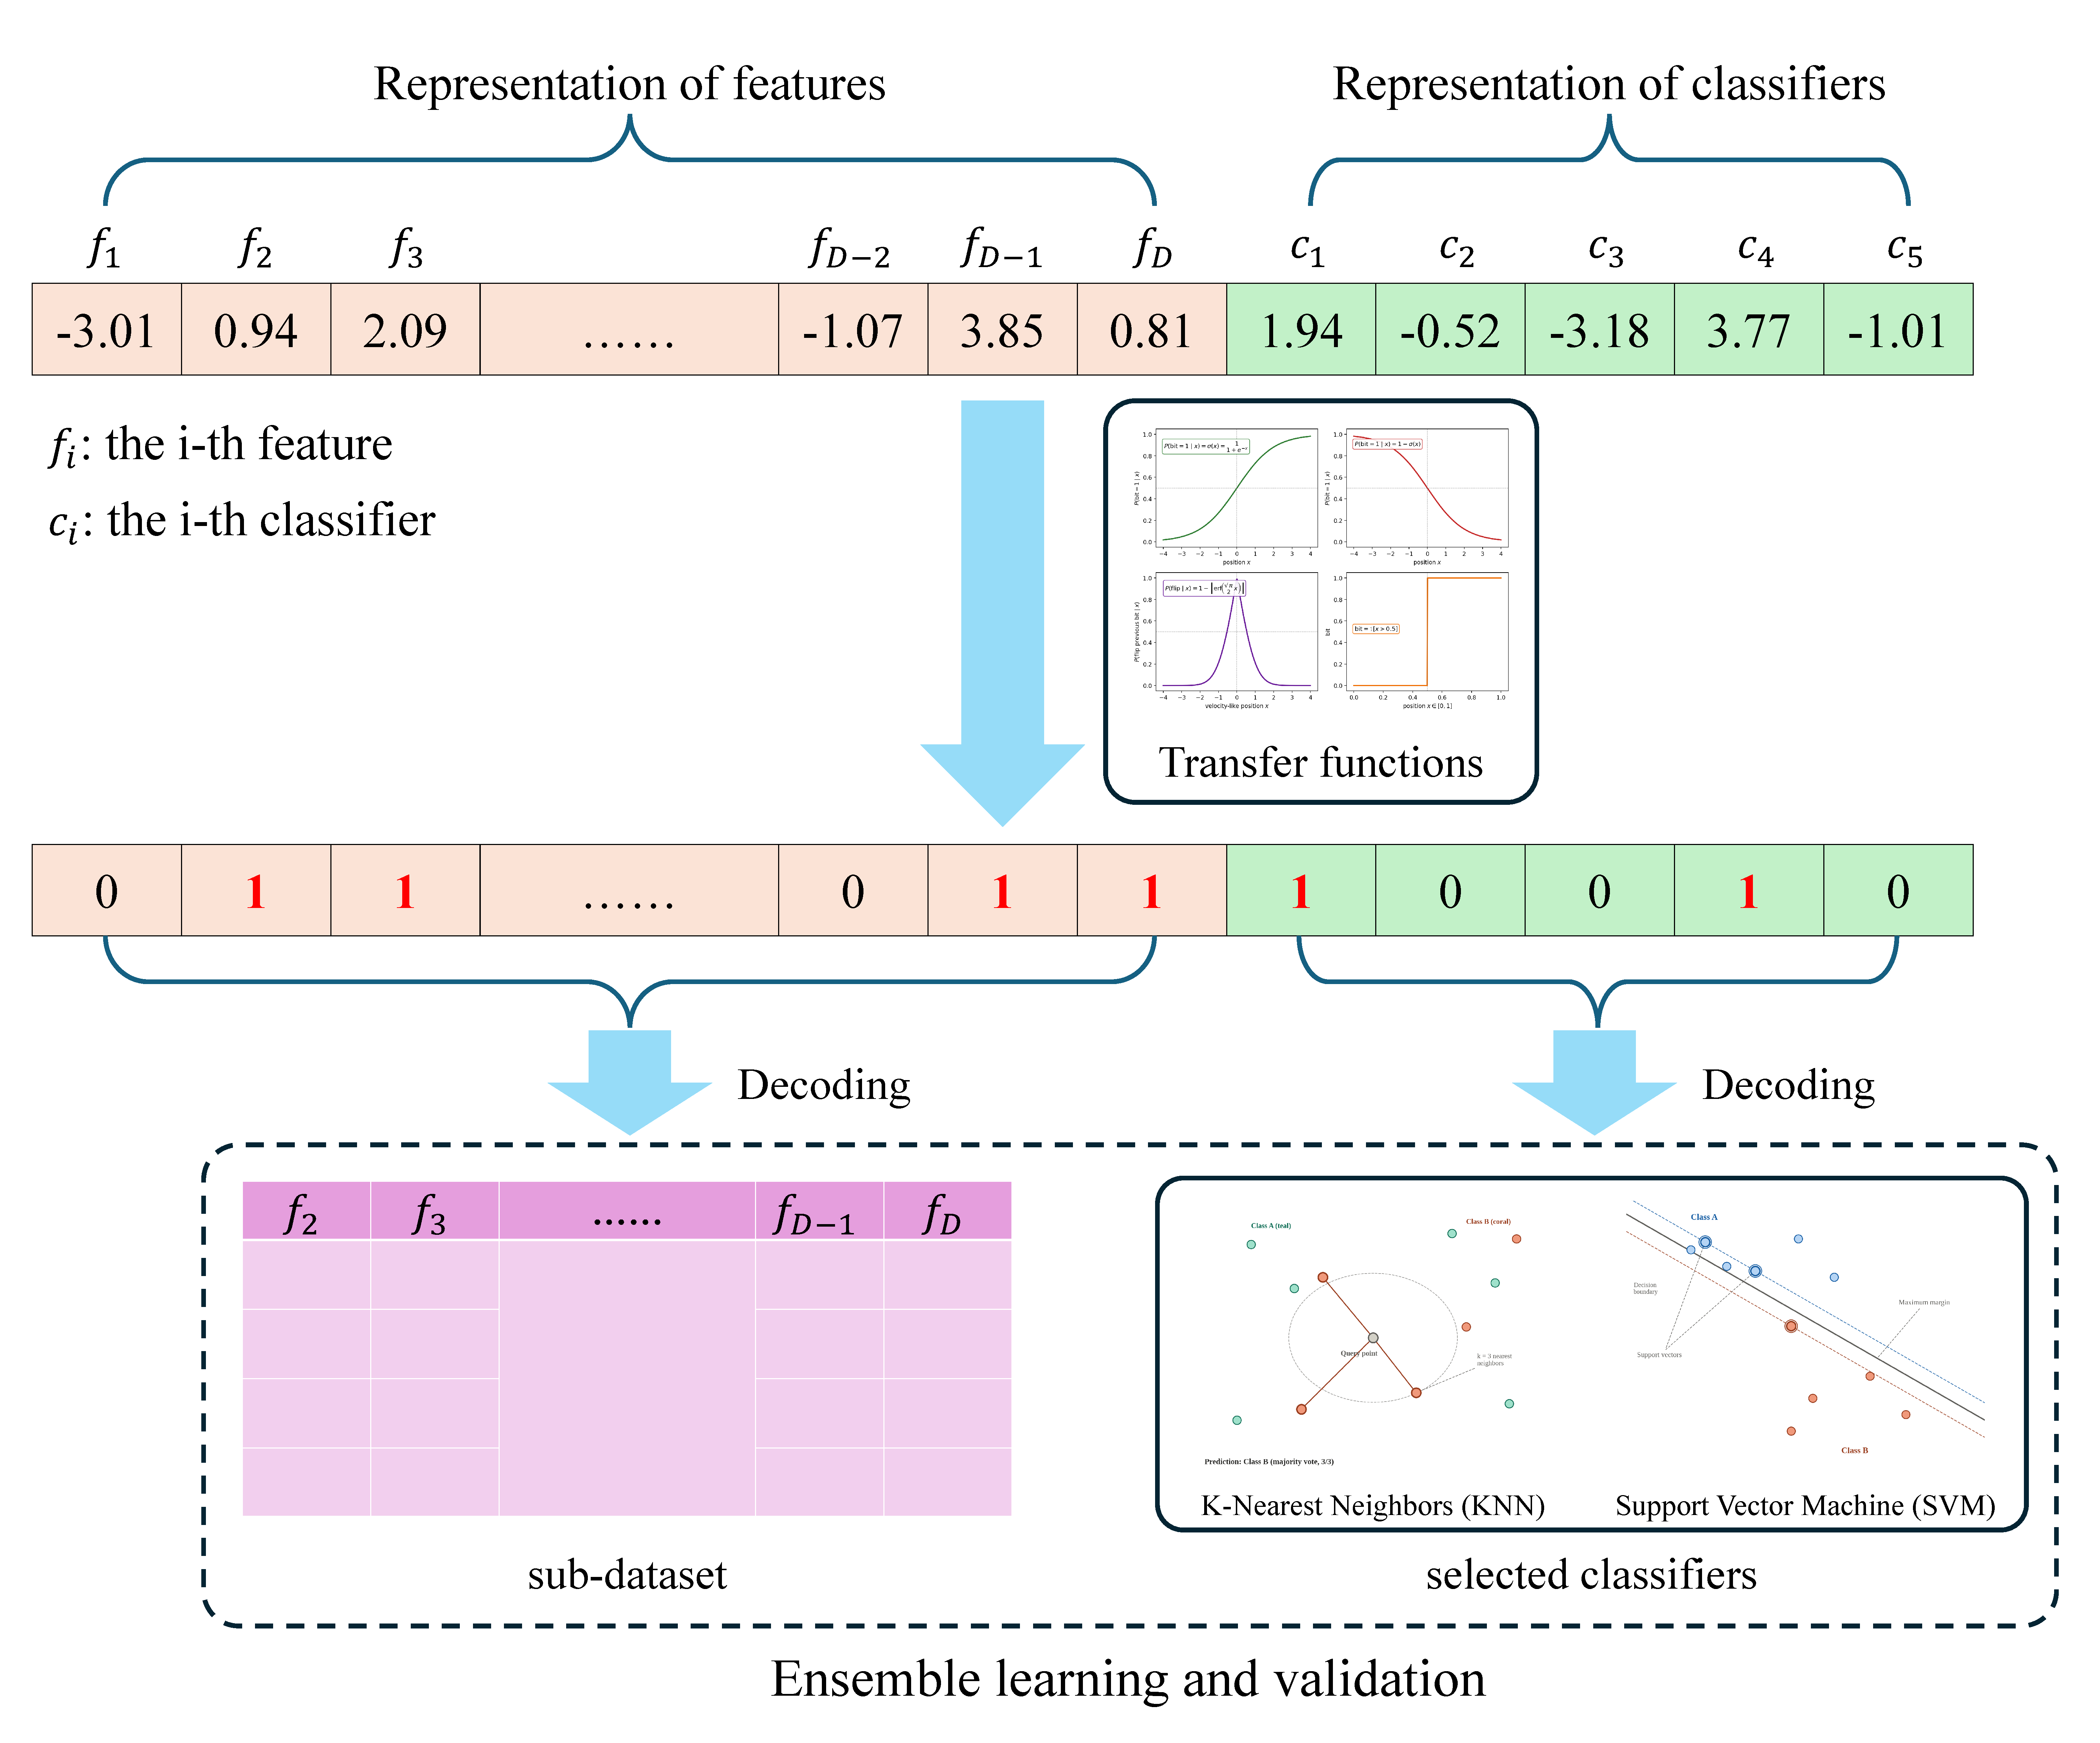
\includegraphics[width=0.95\linewidth]{Encoding.pdf}
  \caption{Worked example of the encoding and decoding pipeline. A continuous particle position of length $5+D+5$ splits into $5$ transfer function scores ($t_1,\dots,t_5$),  $D$ feature scores ($f_1,\dots,f_D$), and 5 classifier scores ($c_1,\dots,c_5$). Each segment passes through a transfer function to produce a binary string; thresholded-off features/classifiers (0) are excluded, and the remainder (1, highlighted) are decoded into a feature mask, here selecting the sub-dataset restricted to columns $f_2, f_3, \ldots, f_{D-1}, f_D$, and a classifier mask, here selecting SVM and KNN. Every classifier in the mask trains on the same feature subset and is combined by equal-weight soft voting before 5-fold subject-grouped cross-validation.}
  \label{fig:3.3.1}
\end{figure}

\subsection{Transfer Functions for Binarization} \label{sec:3.4}
The swarm- and population-based metaheuristics used in this study were, in their original formulation, designed for continuous optimization: a particle's position is a real-valued vector, and the search dynamics, attraction toward better solutions, and so on, are defined in the continuous space. Joint feature-and-classifier selection is inherently discrete, since each dimension of a solution must resolve to a binary decision; that is, a given feature or classifier is either selected or not. A transfer function bridges this mismatch: it maps each continuous position value to a probability or a fixed threshold that determines the corresponding bit, so that an optimizer's continuous-space search dynamics can be reused unchanged while the solution actually evaluated is binary.

Five such transfer functions are adopted in this research, shown in Figure \ref{fig:3.4.1}.
\begin{figure}[t]
  \centering
  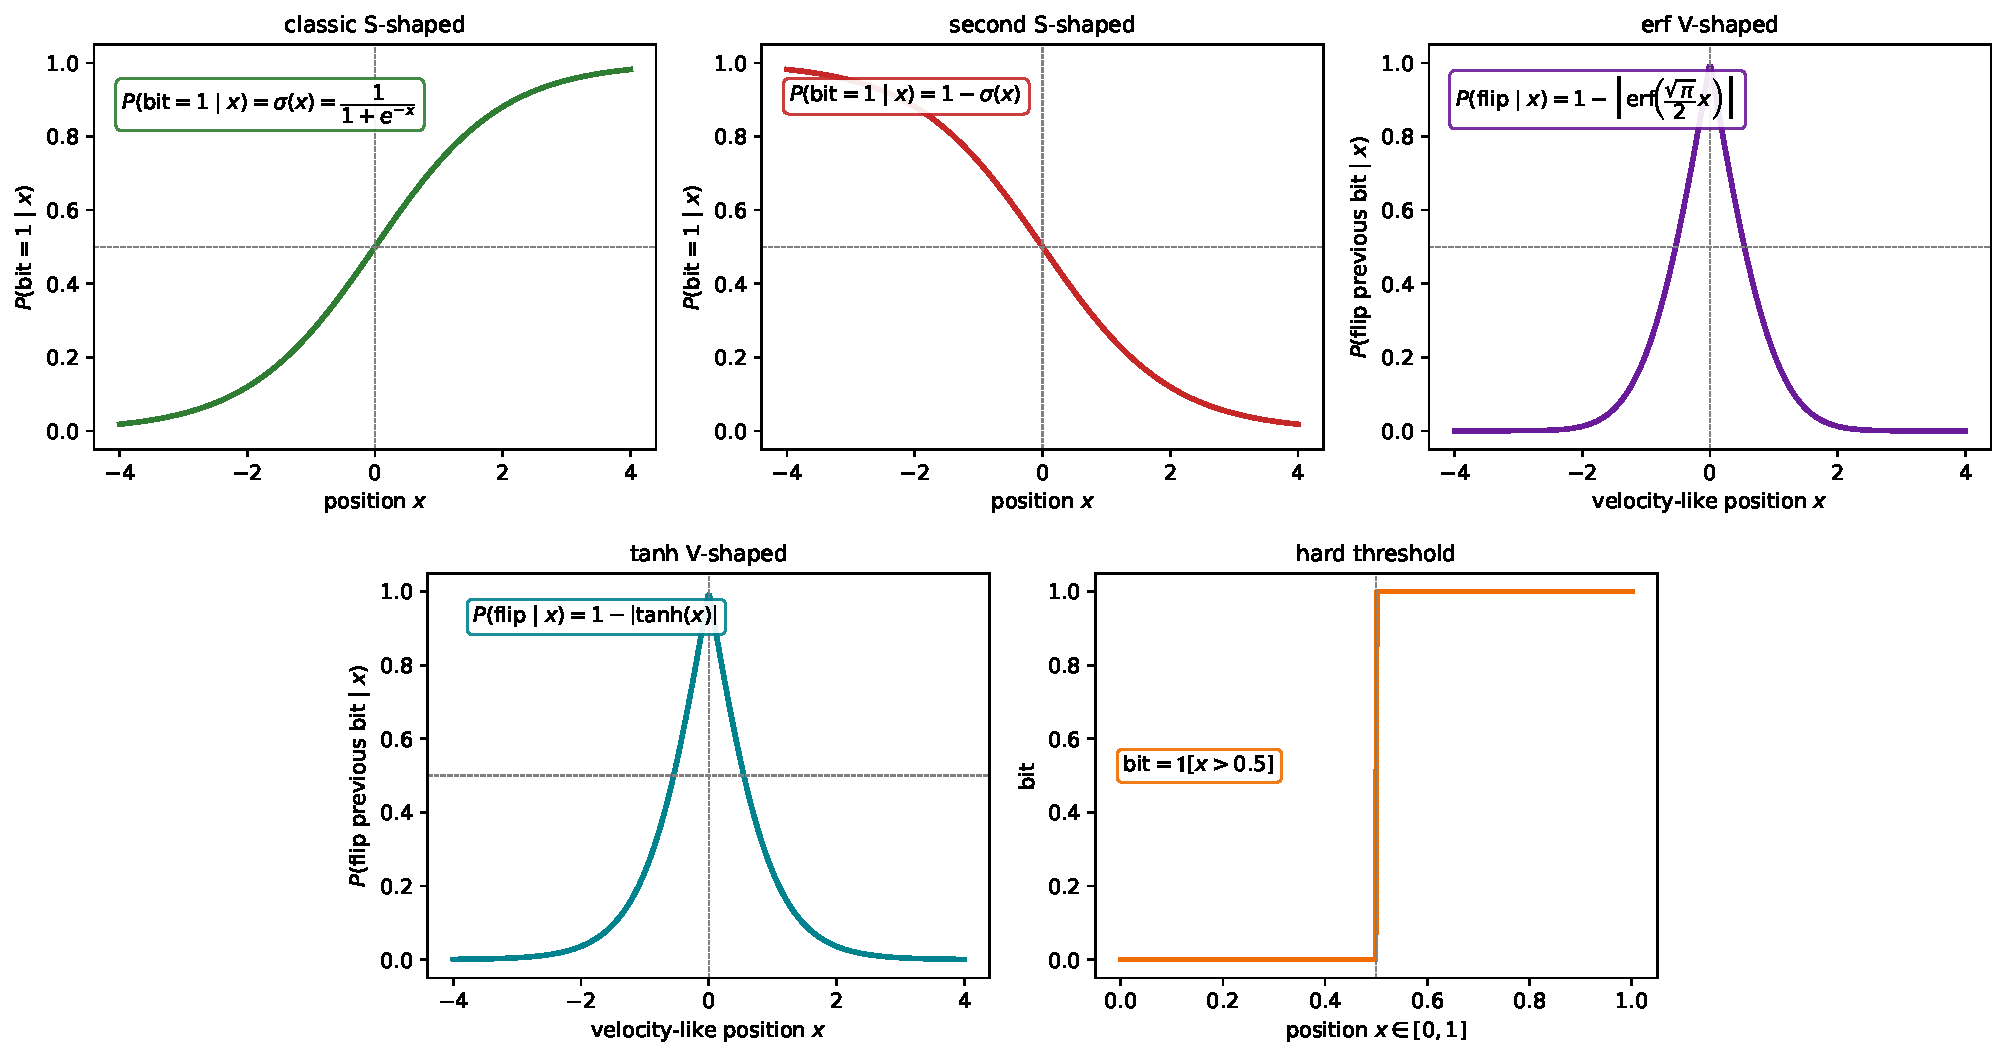
\includegraphics[width=0.95\linewidth]{transfer_functions.pdf}
  \caption{The five transfer functions used in this study: Top row, left to right: classic S-shaped (Eq. (\ref{eq:s-shaped-classic})) \cite{Kuntalp:2024}; second S-shaped (Eq. (\ref{eq:s-shaped-baseline})) \cite{Hashemi:2026}; erf V-shaped (Eq. (\ref{eq:v-shaped})) \cite{Hashemi:2026}. Bottom row, centered under the top row: tanh V-shaped (Eq. (\ref{eq:v-shaped-tanh}) \cite{Mirjalili:2013}; hard threshold (Eq. (\ref{eq:threshold})) \cite{Hashim:2023}, used natively in $[0,1]$.}
  \label{fig:3.4.1}
\end{figure}

The classic stochastic S-shaped transfer function adopts the logistic sigmoid to give the probability that a bit is set, as formulated in Eq. (\ref{eq:s-shaped-classic}).
\begin{equation}
  \sigma(x) = \frac{1}{1 + e^{-x}}, \qquad
  \Pr[\text{bit} = 1] = \sigma(x),
  \label{eq:s-shaped-classic}
\end{equation}
so that selection probability increases monotonically with $x$; this remains an active choice of binarization scheme in recent metaheuristic feature-selection studies \cite{Kuntalp:2024}.

A second S-shaped variant, following Hashemi et al. \cite{Hashemi:2026}, reuses the same logistic sigmoid but decodes in the opposite direction from Eq. (\ref{eq:s-shaped-classic}), which is defined in Eq. (\ref{eq:s-shaped-baseline}).
\begin{equation}
  \Pr[\text{bit} = 1] = 1 - \sigma(x),
  \label{eq:s-shaped-baseline}
\end{equation}
Another V-shaped curve is also defined in \cite{Hashemi:2026} that instead governs whether the previous bit flips, with flip probability in Eq. (\ref{eq:v-shaped}).
\begin{equation}
  \Pr[\text{bit flips}] = 1 - V(x), \qquad
  V(x) = \left| \operatorname{erf}\!\left( \frac{\sqrt{\pi}}{2} x \right) \right|,
  \label{eq:v-shaped}
\end{equation}
which peaks at $x=0$ (where $V(0)=0$) and decays toward 0 as $|x|$ grows (where $V(x) \to 1$).

Besides, a tanh V-shaped curve, following Mirjalili and Lewis's \cite{Mirjalili:2013} own V-shaped family, uses the hyperbolic tangent in place of the error function:
\begin{equation}
  \Pr[\text{bit flips}] = 1 - V_2(x), \qquad
  V_2(x) = |\tanh(x)|,
  \label{eq:v-shaped-tanh}
\end{equation}
with the same flip-the-previous-bit mechanic and the same peaks-at-zero, decays-as-$|x|$-grows shape as Eq. (\ref{eq:v-shaped}), merely a cheaper closed form. Finally, a hard-threshold binarization \cite{Hashim:2023} applies directly to positions that live natively in $[0,1]$, with no stochastic component:
\begin{equation}
  \text{bit} =
  \begin{cases}
    1 & x > 0.5, \\
    0 & \text{otherwise}.
  \end{cases}
  \label{eq:threshold}
\end{equation}

\subsection{Fitness Function} \label{sec:3.5}
Every candidate solution is scored by a single scalar fitness, combining diagnostic performance with a feature-parsimony penalty in Eq. (\ref{eq:3.5.1}):
\begin{equation}
  \text{fitness} = \omega \cdot (1 - \text{BalAcc}) + (1 - \omega) \cdot \frac{|S|}{D}
  \label{eq:3.5.1}
\end{equation}
where $\text{BalAcc}$ is the out-of-fold balanced accuracy (the average of sensitivity and specificity, robust to Oxford's class imbalance \cite{Brodersen:2010}) achieved by the decoded feature subset and ensemble of classifiers, $|S|$ is the number of selected features, $D$ is the total number of available features, and $\omega = 0.9$ weights diagnostic performance nine times as heavily as feature count, as suggested in \cite{Priyadharshini:2024}. This value ensures a modest reduction in feature count is rewarded only when it does not come at a material cost to balanced accuracy. Additionally, lower fitness is better, and every optimizer in this study is implemented as a minimizer.


\subsection{Our Proposed Pipeline: The Joint Optimization via Competitive Swarm Optimizer} \label{sec:3.6}
The contribution of this study is not a new metaheuristic operator but a new paradigm for handling metaheuristic-based feature selection efficiently. As reviewed in Section \ref{sec:2.3}, published metaheuristic pipelines for PD voice screening almost universally treat the transfer function, the feature subset, and the classifier configuration as three separate decisions, of which only the feature subset is determined via metaheuristic search, while the other two components are configured by hand according to expert judgment. This section describes the pipeline that instead searches all three jointly, within the single $5+D+5$-dimensional encoding of Section \ref{sec:3.3} and the fitness of Section \ref{sec:3.5}, using the Competitive Swarm Optimizer (CSO) \cite{Cheng:2015} as the search engine that explores this space generation by generation.

\subsubsection{Basic CSO} \label{sec:3.6.1}
The Competitive Swarm Optimizer (CSO) was originally proposed by Cheng and Jin in 2015 \cite{Cheng:2015}, which departs from the attractor-based update rule common to PSO, where every particle is pulled toward the personal best and global best solution. CSO instead structures each generation as a set of pairwise competitions: only the loser of each pair updates and learns from the winner particle and the centroid position. This design is intended to preserve swarm diversity and allocate the computational budgets to the promising solutions. Concretely, in each generation, the even-numbered population of $N$ particles is randomly paired into $N/2$ one-on-one competitions. Within each pair, the fitter particle, denoted as $\bm{v}^t_w$, passes to the next generation unchanged, while the weaker particle, denoted as $\bm{v}^t_l$, updates its velocity and position toward the winner and the centroid of the swarm, as described in Eq. (\ref{eq:3.6.1}):
\begin{equation}
    \label{eq:3.6.1}
    \begin{aligned}
        & \bm{v}^{t+1}_l = \bm{R}_1 \cdot \bm{v}^t_l + \bm{R}_2 \cdot (\bm{x}^t_w - \bm{x}^t_l) + \varphi \cdot \bm{R}_3 \cdot (\bar{\bm{x}}^t - \bm{x}^t_l) \\
        & \bm{x}^{t+1}_l = \bm{x}^t_l + \bm{v}^{t+1}_l
    \end{aligned}
\end{equation}
where $\bm{x}^t_w$ and $\bm{x}^t_l$ are the winner's and loser's positions, respectively, $\bar{x}$ is the centroid of the swarm, $\bm{R}_1$, $\bm{R}_2$, and $\bm{R}_3$ are independent uniform random vectors, and $\phi$ is CSO's social-term control coefficient, where the sensitivity analysis for $\phi$ in this specific joint optimization task is provided in Section \ref{sec:sensitivity}.


\subsubsection{The Implementation of Our Proposed Framework} \label{sec:3.6.2}
Figure \ref{fig:3.6.2.1} traces one full generation of the proposed pipeline end-to-end, tying together the encoding of Section \ref{sec:3.3}, the transfer-function candidates of Section \ref{sec:3.4}, the CSO update of Section \ref{sec:3.6.1}, and the fitness of Section \ref{sec:3.5} into the single procedure that this study actually runs.
\begin{figure}[t]
  \centering
  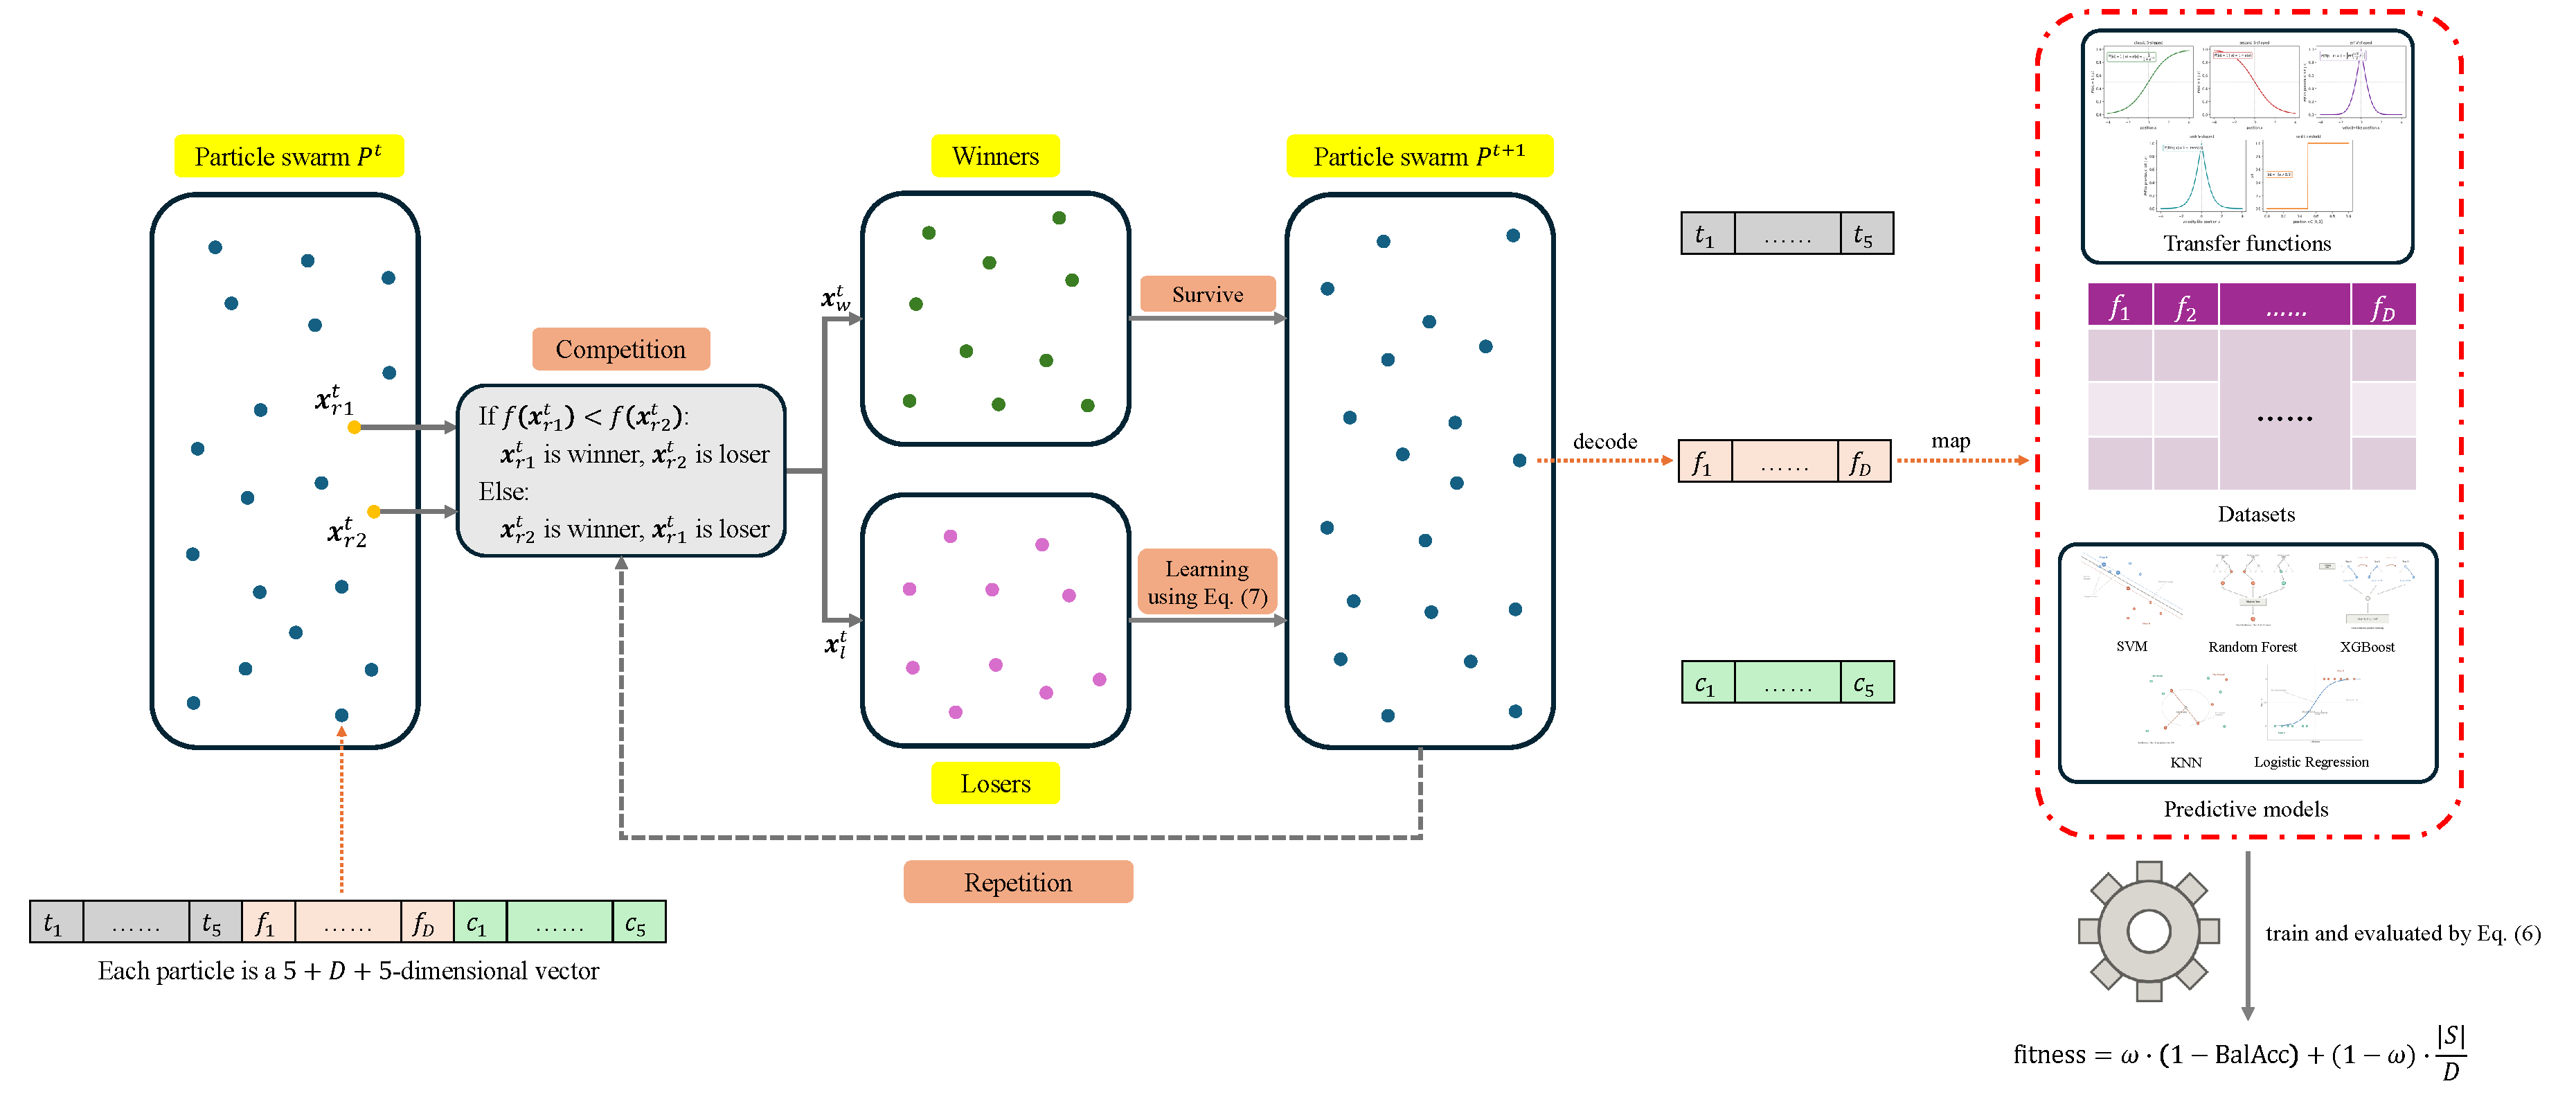
\includegraphics[width=0.95\linewidth]{CSO.pdf}
  \caption{One full generation of the proposed pipeline.}
  \label{fig:3.6.2.1}
\end{figure}

Each particle in the swarm $P^t$ is a $5+D+5$-dimensional vector $[t_1,\ldots,t_5, f_1,\ldots,f_D, \\c_1,\ldots,c_5]$. Every generation, particles are randomly paired and compared based on the competition mechanism in CSO; each pair's winner survives unchanged into $P^{t+1}$, while its loser's entire position is updated by Eq. (\ref{eq:3.6.1}) before being decoded and re-evaluated. Decoding a position for the updated particle individual consists of three steps:
\begin{enumerate}
  \item \textbf{Transfer-function selection}: The leading segment $[t_1,\ldots,t_5]$ is argmaxed to pick one of the 5 candidate transfer functions without a binarization step.
  \item \textbf{Feature and classifier mapping}: The selected candidate binarizes the trailing $[f_1,\ldots,f_D,\\ c_1,\ldots,c_5]$ segment based on the specific transfer function. The resulting $D$-bit feature mask selects which of the dataset's $D$ acoustic-feature columns are retained (map in Figure \ref{fig:3.6.2.1}); the resulting 5-bit classifier mask selects which of the five candidate classifiers are included in that particle's ensemble.
  \item \textbf{Training and evaluation}:  The selected classifiers are trained on the selected feature subset under the subject-grouped cross-validation protocol of Section \ref{sec:3.2} and combined into an equal-weight soft-voting ensemble; the resulting out-of-fold balanced accuracy and feature ratio are combined into the scalar fitness computed by Eq. (\ref{eq:3.5.1}).
\end{enumerate}
The resulting fitness value is what determines that particle's winner/loser status the next time it is paired, closing the loop shown at the bottom of Figure \ref{fig:3.6.2.1}: decode, map, train, and evaluate happen every time a loser updates, generation after generation, for every particle in the swarm.

\subsection{Comparison Methods} \label{sec:3.7}
Five metaheuristic feature-selection methods from recently published papers, specifically focus on PD diagnosis, are re-implemented to enable a controlled, like-for-like comparison against the proposed framework: binary grey wolf optimizer (BGWO) and a whale-optimization-then-grey-wolf refinement cascade (HybridGWO) \cite{AlNajjar:2024}, mayfly algorithm with a quantum-rotation-gate mutation operator (QMFO)\cite{Mansour:2024}, and binary particle swarm optimization (BPSO) as well as butterfly optimization algorithm (BBOA) with a hybrid S-shaped or V-shaped transfer function \cite{Hashemi:2026}.
\begin{table}[t]
  \centering
  \renewcommand{\arraystretch}{1.2}
  \caption{Hyperparameters of algorithms.}
  \label{tab:hyperparameters}
  \begin{tabular}{ll}
    \toprule
    Algorithm & Hyperparameters \\
    \midrule
    BGWO & $a: 2\to0$ \\
    HybridGWO & WOA: $b=1.0$; GWO: $a: 2\to0$  \\
    QMFO & $a_1=1.0$, $a_2=1.5$, $\beta=2.0$, $\text{dance}=5.0$, \\
    ~ & $fl=1.0$, rotation step $=0.15$ \\
    BPSO & $w=0.7$, $c_1=2.5$, $c_2=1.6$ \\
    BBOA & $c=0.01$, $a \in [0.1, 0.3]$, $p=0.6$  \\
    CSO & $\varphi=0$ (As recommended in \cite{Cheng:2015} that when $N<100$, $\varphi=0$)  \\
    \bottomrule
  \end{tabular}
\end{table}

Every optimizer is compared under an equal fitness-evaluation budget ($FE_{max}$) rather than an equal generation count, since different algorithms consume different numbers of fitness evaluations per generation (e.g., the hybrid S-shaped/V-shaped transfer function used by BPSO/BBOA evaluates two binarization candidates per individual per generation; mHGS's production and escaping operators each conditionally trigger additional evaluations). A population size of 30 and a fitness-evaluation budget of $FE_{max} = 3000$ per run are used throughout. Each algorithm-dataset combination is run with multiple independent seeds (seed $= 2026 + 50 \times i$, where $i$ is the run index in $\{1, 2, \dots, 50\}$, so seeds do not overlap across runs). This fair and detailed comparison against the five baselines, carried out across multiple environments, uses enough independent runs to support the statistical testing described in Section \ref{sec:4}.


\subsection{Evaluation Metrics} \label{sec:3.8}
For every run, the out-of-fold predictions used to compute fitness are also used to report a full panel of standard diagnostic-performance metrics, computed once per run from the same confusion matrix, whose entries are true positives (TP), true negatives (TN), false positives (FP), and false negatives (FN), with the Parkinsonian class taken as positive:
\begin{align}
  \text{Accuracy} &= \frac{TP + TN}{TP + TN + FP + FN} \label{eq:accuracy} \\
  \text{Sensitivity (Recall)} &= \frac{TP}{TP + FN} \label{eq:sensitivity} \\
  \text{Specificity} &= \frac{TN}{TN + FP} \label{eq:specificity} \\
  \text{BalAcc} &= \frac{\text{Sensitivity} + \text{Specificity}}{2} \label{eq:balanced-accuracy} \\
  \text{Precision} &= \frac{TP}{TP + FP} \label{eq:precision} \\
  \text{F1} &= 2 \cdot \frac{\text{Precision} \cdot \text{Sensitivity}}{\text{Precision} + \text{Sensitivity}} \label{eq:f1} \\
  \text{ROC-AUC} &= \Pr\big(\hat{p}(x^+) > \hat{p}(x^-)\big) \label{eq:roc-auc}
\end{align}
where $\hat{p}(x)$ is the predicted probability of the Parkinsonian class for a recording $x$, and $x^+$, $x^-$ are independently drawn Parkinsonian and healthy-control recordings, respectively. That is, ROC-AUC, formulated in Eq. (\ref{eq:roc-auc}), is the probability that the model ranks a randomly drawn positive case above a randomly drawn negative one, equivalently the area under the curve traced by the true positive rate versus the false positive rate as the decision threshold varies, unlike Eqs. (\ref{eq:accuracy}) to (\ref{eq:f1}), which are all evaluated at the single decision threshold ($0.5$) used elsewhere in this study. Sensitivity and specificity are reported alongside the more ML-conventional accuracy/F1/AUC metrics because they are the standard vocabulary for evaluating a clinical screening tool: sensitivity in Eq. (\ref{eq:sensitivity}) quantifies the fraction of true PD cases the pipeline would flag (missed cases have direct clinical cost), while specificity in Eq. (\ref{eq:specificity}) quantifies the fraction of healthy individuals correctly spared unnecessary follow-up. $\text{BalAcc}$ in Eq. (\ref{eq:balanced-accuracy}) is the same quantity used inside the fitness function, so the primary search objective and the headline reported metric are one and the same, not two different notions of accuracy. Feature-selection ratio ($|S|/D$) and the active classifier(s) are also recorded for every run; the identity of the specific features selected is not logged in the current experiment pipeline, which Section \ref{sec:5} discusses as a limitation to be addressed before a feature-interpretability analysis is possible.
